

\subsection{Marking Externalization Snippets\\标记外部化代码片段}\label{subsec:external_marking}

\begin{docEnvironment}[doc new=2015-03-11]{tcbexternal}{\oarg{options}\marg{name}}
Marks the environment content as a snippet for externalization.
Typically, the content is a |tikzpicture| or something similar.
It is important to note that the snippet should not have any dependencies
with the rest of the document, e.g. referencing counters or setting counters
is not possible.

将环境内容标记为外部化片段。通常,内容是一个 |tikzpicture| 或类似的东西。需要注意的是,片段不应与文档的其他部分有任何依赖关系,例如引用计数器或设置计数器是不可能的。

The \meta{name} is automatically prefixed with \refKeyLe{/tcb/external/prefix}.
In combination, this has to be a unique file name. It is advised to not
use spaces or umlauts for the name.
The \meta{options} are keys from the |/tcb/external/| key tree.

\meta{name}会自动加上 \refKeyLe{/tcb/external/prefix},二者组合后必须是一个唯一的文件名。建议不要在名称中使用空格或umlauts。 \meta{options} 是 |/tcb/external/| 关键字树中的键。
\begin{dispExample}
\begin{tcbexternal}{example_tikzpicture}
  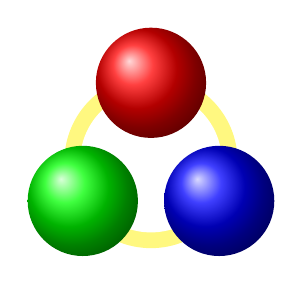
\begin{tikzpicture}
    \path[fill=yellow!50!white] (0,0) circle (11mm);
    \path[fill=white] (0,0) circle (9mm);
    \foreach \w/\c in {90/red,210/green,330/blue}
      {\path[shading=ball,ball color=\c] (\w:1cm) circle (7mm);}
  \end{tikzpicture}
\end{tcbexternal}
\end{dispExample}


% \medskip

If a \refEnvLe{tcolorbox} is externalized, one should use
\refKeyLe{/tcb/nobeforeafter} for the box. Indention and distances to
the text before and after have to be given separately outside the
\refEnvLe{tcbexternal} environment.

如果要外部化一个\refEnvLe{tcolorbox},则应使用\refKeyLe{/tcb/nobeforeafter}进行框架。缩进和文本之前和之后的距离必须在\refEnvLe{tcbexternal}环境外分别给出。
\begin{dispExample}
\noindent%
\begin{tcbexternal}[minipage]{example_tcolorbox}
  \begin{tcolorbox}[nobeforeafter,enhanced,
      fonttitle=\bfseries,title=Externalized Box,
      colframe=red!50!black,drop fuzzy shadow,
      interior style={fill overzoom image=goldshade.png}]
This complete tcolorbox is externalized. One cannot use numbered
boxes here. Note the \texttt{minipage} option which tells the
current line width to the external snippet.

这个完整的 |tcolorbox| 被外部化了。在这里无法使用编号的盒子。请注意,\texttt{minipage} 选项告诉外部片段当前的行宽度。
\end{tcolorbox}
\end{tcbexternal}
\end{dispExample}

\begin{dispExample}
\begin{tcolorbox}[nobeforeafter,enhanced,
      fonttitle=\bfseries,title=Externalized Box,
      colframe=blue!50!black,
      interior style={fill overzoom image=blueshade.png}]
\begin{tcbexternal}[minipage]{example_tcolorbox2}
\color{white}%
The interior of the tcolorbox is externalized.
One can use numbered boxes without problems.
Note that the text color has to be set for the text manually
since it is converted into an image.

这个 |tcolorbox| 的内部被外部化了。可以无问题地使用带编号的盒子。请注意,由于文本被转换成图像,所以必须手动设置文本的颜色。
\end{tcbexternal}
\end{tcolorbox}
\end{dispExample}



\begin{dispExample}
\begin{tcbexternal}[minipage]{example_tabularx}
  \newcolumntype{Y}{>{\raggedleft\arraybackslash}X}%
  \begin{tabularx}{\linewidth}{|l||Y|Y|Y|Y||Y|}\hline
    Group & One & Two & Three & Four & Sum\\\hline\hline
    Red & 1000.00 & 2000.00 & 3000.00 & 4000.00 & 10000.00\\\hline
    Green & 2000.00 & 3000.00 & 4000.00 & 5000.00 & 14000.00\\\hline
    Blue & 3000.00 & 4000.00 & 5000.00 & 6000.00 & 18000.00\\\hline\hline
    Sum & 6000.00 & 9000.00 & 12000.00 & 15000.00 & 42000.00\\\hline
  \end{tabularx}
\end{tcbexternal}
\end{dispExample}
\end{docEnvironment}

\begin{extTcbKey}[][doc new=2015-03-11]{name}{=\meta{name}}{no default,
  initially \texttt{unnamed}}
The \meta{name} is automatically prefixed with \refKeyLe{/tcb/external/prefix}.
In combination, this has to be a unique file name for externalization.
Typically, this key is not used directly but is set indirectly as
mandatory parameter, see \refEnvLe{tcbexternal}.

\meta{name} 会自动加上前缀 \refKeyLe{/tcb/external/prefix},两者组合后成为用于外部化的唯一文件名。通常情况下,这个键不会被直接使用,而是间接设置为必填参数,参见 \refEnvLe{tcbexternal}。
\end{extTcbKey}

% \clearpage
\begin{docEnvironment}[doc new=2015-03-11]{extcolorbox}{\oarg{options}\marg{name}\oarg{tcolorbox options}}
This is an externalized version of \refEnvLe{tcolorbox} created
using\\ \refComLe{newtcbexternalizetcolorbox}:

这是使用 \refComLe{newtcbexternalizetcolorbox} 创建的 \refEnvLe{tcolorbox} 的外部化版本:
\begin{dispListing}
\newtcbexternalizetcolorbox{extcolorbox}{tcolorbox}{}{}
\end{dispListing}
\meta{options} and \meta{name} are given to the underlying \refEnvLe{tcbexternal}
environment, while \meta{tcolorbox options} are given to \refEnvLe{tcolorbox}.

\meta{options} 和 \meta{name} 会传递给基础的 \refEnvLe{tcbexternal} 环境,
而 \meta{tcolorbox options} 会传递给 \refEnvLe{tcolorbox}。

\begin{marker}
Note that you should not redefine \refKeyLe{/tcb/before} and \refKeyLe{/tcb/after}
inside the \meta{tcolorbox options}, since the
externalized version would not be identical to the non-externalized
otherwise.

请注意,不要在 \meta{tcolorbox options} 中重新定义 \refKeyLe{/tcb/before} 和 \refKeyLe{/tcb/after},否则外部化版本将与非外部化版本不相同。
\end{marker}

\begin{dispExample}
\begin{extcolorbox}[minipage]{example_extcolorbox}
[ enhanced,colframe=red!50!black,colback=yellow!10,
fonttitle=\bfseries,drop fuzzy shadow,
title=My external box ]

This box is completely externalized.

这个盒子完全被外部化了。

\begin{tcolorbox}[colframe=blue,colback=blue!5,before skip=6pt]
Inner box.

内部盒子。
\end{tcolorbox}
\end{extcolorbox}
\end{dispExample}
\end{docEnvironment}

\begin{marker}
\begin{itemize}
\item\textbf{Never} externalize numbered boxes.

\textbf{永远不要}将带有编号的盒子外部化。
\item\textbf{Never} externalize boxes which contain references to other
  things, e.g. using |\ref| or |\cite|.

\textbf{永远不要}将带有对其他内容引用的盒子(例如使用$|\ref|$ 或 $|\cite|$)外部化。
  \item\textbf{Never} externalize breakable boxes.

\textbf{永远不要}将可断行的盒子外部化。\end{itemize}
\kern6pt
\end{marker}

% \clearpage
\begin{docEnvironment}[doc new=2015-03-11]{extikzpicture}{\oarg{options}\marg{name}\oarg{tikz options}}
This is an externalized version of |tikzpicture| created
using\\ \refComLe{newtcbexternalizeenvironment}:

这是一个使用 \refComLe{newtcbexternalizeenvironment} 创建的 |tikzpicture| 的外部化版本:
\begin{dispListing}
\newtcbexternalizeenvironment{extikzpicture}{tikzpicture}{}{}{}
\end{dispListing}
\meta{options} and \meta{name} are given to the underlying \refEnvLe{tcbexternal}
environment, while \meta{tikz options} are given to |tikzpicture|.

\meta{options} 和 \meta{name} 将传递给底层的 \refEnvLe{tcbexternal} 环境,而 \meta{tikz options} 将传递给 |tikzpicture|。
\tcbset{/tcb/external/externalize}%----- Do externalization even if switched off globally
\begin{dispExample}
\begin{center}
\begin{extikzpicture}[
  preamble={\usepackage{pgfplots}},  % add package for external graph
  input source on error=false,       % do not load source on error
]{example_pgfplots}
  \pgfplotsset{width=12cm}
  \begin{axis}[3d box=background,grid=major,
    xlabel=$x$, ylabel=$y$, zlabel=$z$, view/h=40,
    mesh/interior colormap name=hot,
    colormap/blackwhite,
    z buffer=sort,domain=0:90,y domain=0:60,
    zmin=0,zmax=2,z post scale=1.2,
    ]
  \addplot3[surf,mesh/interior colormap name=blackwhite,
    colormap/hot,] ( {cos(x)},{sin(x)}, {2*sin(y)} );
  \addplot3[surf] ( {2*cos(x)*cos(y)},{2*sin(x)*cos(y)}, {2*sin(y)} );
  \end{axis}
\end{extikzpicture}
\end{center}
\end{dispExample}

\end{docEnvironment}




% \clearpage
\begin{docTcbKey}[][doc new=2015-03-11]{externalize listing}{=\meta{name}}{style, no default}
The text content of a \refEnvLe{tcblisting} is externalized with the
given \meta{name}. Note that the listing part is not externalized.

使用给定的\meta{name}将\refEnvLe{tcblisting}的文本内容外部化。请注意,代码部分不会被外部化。
\end{docTcbKey}

\begin{dispExample}
\begin{tcblisting}{externalize listing=example_listing,
  bicolor,colback=yellow!10,colframe=yellow!50!black,
  colbacklower=white,center lower}
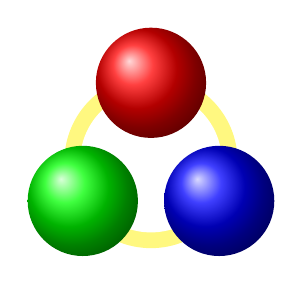
\begin{tikzpicture}
  \path[fill=yellow!50!white] (0,0) circle (11mm);
  \path[fill=white] (0,0) circle (9mm);
  \foreach \w/\c in {90/red,210/green,330/blue}
    {\path[shading=ball,ball color=\c] (\w:1cm) circle (7mm);}
\end{tikzpicture}
\end{tcblisting}
\end{dispExample}


\begin{docTcbKey}[][doc new=2015-03-11]{externalize listing\tcbexclamation}{=\meta{name}}{style, no default}
Combination of \refKeyLe{/tcb/externalize listing} and \refKeyLe{/tcb/external/force remake}.

\refKeyLe{/tcb/externalize listing} 和 \refKeyLe{/tcb/external/force remake} 的组合。
\end{docTcbKey}

\begin{docTcbKey}[][doc new=2015-03-11]{externalize example}{=\meta{name}}{style, no default}
The text content of a \refEnvLe{dispExample*} is externalized with the
given \meta{name}. Note that the listing part is not externalized.

使用给定的\meta{name}将\refEnvLe{dispExample*}的文本内容外部化。请注意,代码部分不会被外部化。
\begin{dispExample}
\begin{dispExample*}{sidebyside,externalize example=example_example}
\tikz\path[shading=ball,
  ball color=red] circle (7mm);
\end{dispExample*}
\end{dispExample}
\end{docTcbKey}

\begin{docTcbKey}[][doc new=2015-03-11]{externalize example\tcbexclamation}{=\meta{name}}{style, no default}
Combination of \refKeyLe{/tcb/externalize example} and \refKeyLe{/tcb/external/force remake}.

\refKeyLe{/tcb/externalize example} 和 \refKeyLe{/tcb/external/force remake} 的组合。
\end{docTcbKey}